% Bank-size heterogeneity in quarterly changes: figures and distributional commentary.
% Figures and tables are produced by notebooks/descriptive_figures.ipynb; re-run it before compiling.
\documentclass[11pt]{article}

\usepackage[margin=1in]{geometry}
\usepackage[T1]{fontenc}
\usepackage{newtxtext,newtxmath}   % Times, matching the figure typeface
\usepackage{amsmath}
\usepackage{graphicx}
\usepackage{booktabs}
\usepackage{float}
\usepackage[font=small,labelfont=bf,labelsep=period,justification=justified,singlelinecheck=false]{caption}
\usepackage{threeparttable}
\usepackage{enumitem}
\usepackage[hidelinks]{hyperref}

\graphicspath{{../output/figures/}}
\newcommand{\tablepath}{../output/tables}
\setlength{\parskip}{0.4em}
\setlist{itemsep=0.25em, topsep=0.3em}

\title{Initial Data Assessment:\\
       Distributions of Quarterly Changes by Bank Size, 1992--2026}
\author{William Rouse}
\date{\today}

\begin{document}
\maketitle

\begin{abstract}
\noindent
This note documents how the cross-sectional distributions of four bank outcomes---total assets, the equity-to-assets ratio, return on assets (ROA), and net interest margin (NIM)---change over one-, two-, and three-quarter horizons, separately for the largest 1\% of FDIC-insured institutions and for all other banks. The distributions are roughly symmetric around zero during expansions. During recessions they widen and develop a negative skew in capital and profitability. The largest banks show the sharper swings in median ROA and the larger increase in dispersion.
\end{abstract}

\section{Data and construction}\label{sec:data}

The sample is the FDIC Statistics on Depository Institutions bank-quarter panel from 1992Q1 to 2026Q2, with 1{,}129{,}925 bank-quarters and 17{,}161 institutions identified by FDIC certificate number. In each quarter $t$, banks are ranked by total assets. The top 1\% form the \emph{large-bank} group (between 42 and 144 institutions, depending on the year) and the remaining 99\% form the \emph{other-bank} group. Group membership is re-assigned every quarter.

For bank $i$ and horizon $k \in \{1,2,3\}$, the outcome is the change from quarter $t-k$ to quarter $t$, matched on the same institution:
\begin{align*}
  \Delta_k A_{it} &= 100 \times \left( A_{it} / A_{i,t-k} - 1 \right) && \text{(total assets, percent)} \\
  \Delta_k x_{it} &= x_{it} - x_{i,t-k} && \text{(equity/assets, ROA, NIM; percentage points)}
\end{align*}
Asset changes are expressed in percent because dollar changes are not comparable across institutions whose balance sheets differ by several orders of magnitude.

The FDIC reports ROA and NIM year-to-date and annualized, so differencing them directly would compare a single quarter with a full year every first quarter. Each bank's single-quarter ratio is therefore recovered first:
\[
  r^{q}_{Q} = Q \cdot r^{\mathrm{ytd}}_{Q} - (Q-1) \cdot r^{\mathrm{ytd}}_{Q-1}, \qquad r^{q}_{1} = r^{\mathrm{ytd}}_{1},
\]
within each calendar year, where $Q$ is the quarter of the year. The formula is exact when average assets are stable within the year and a close approximation otherwise.

Figures~\ref{fig:assets}--\ref{fig:nim} are fan charts. In each quarter, the line marks the median change across banks in the group, the dark band the 25th--75th percentiles, and the light band the 10th--90th percentiles. Rows correspond to the horizon $k$, and all six panels in a figure share one vertical axis. Gray shading marks NBER recessions.

% ---------------------------------------------------------------------------
% Figures (float pages; flushed by the \clearpage before Section 2)

\begin{figure}[p]
  \centering
  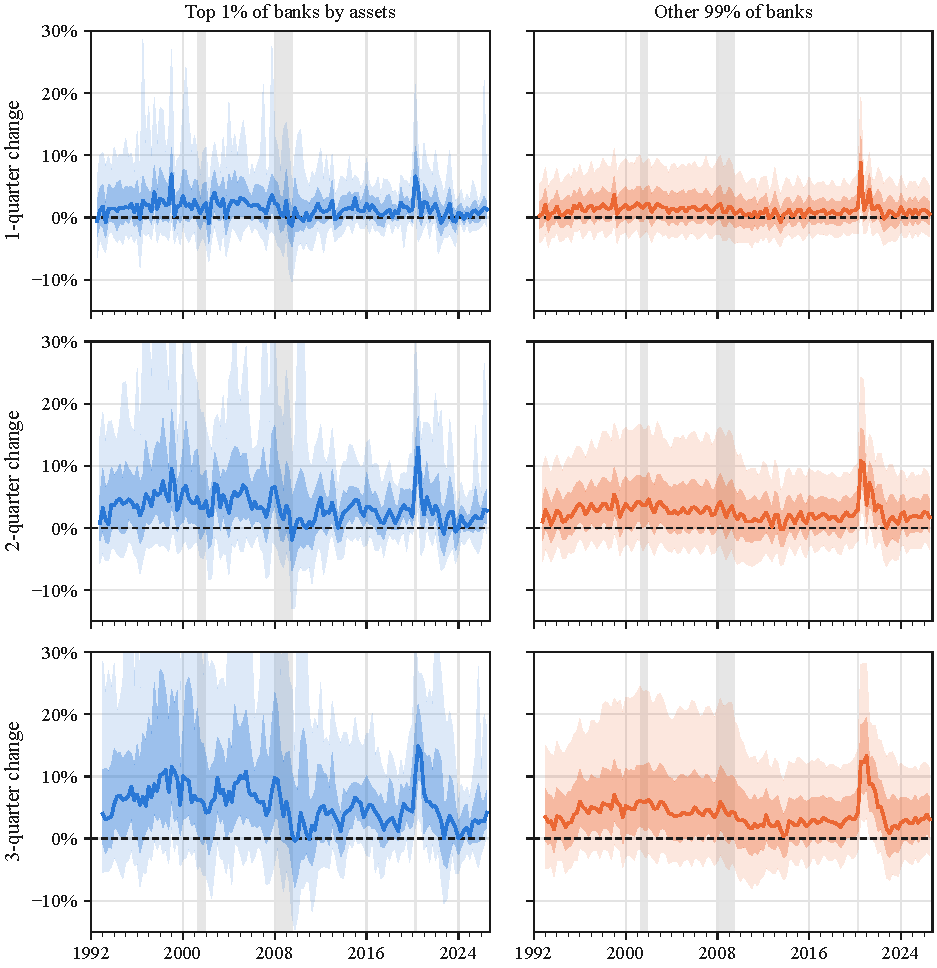
\includegraphics[width=\textwidth]{size_diff_assets_bare.pdf}
  \caption{Change in total assets (percent).}
  \label{fig:assets}
  \vspace{0.2em}
  \begin{minipage}{\textwidth}\footnotesize
    \textit{Notes:} Percent change in each bank's total assets from $k$ quarters earlier. Changes include mergers and acquisitions. The vertical axis is capped at $-15\%$ and $30\%$; the large-bank upper tail exceeds $100\%$ in several late-1990s quarters. Line: median bank; dark band: 25th--75th percentiles; light band: 10th--90th percentiles. Shaded areas indicate NBER recessions. \textit{Source:} FDIC Statistics on Depository Institutions; author's calculations.
  \end{minipage}
\end{figure}

\begin{figure}[p]
  \centering
  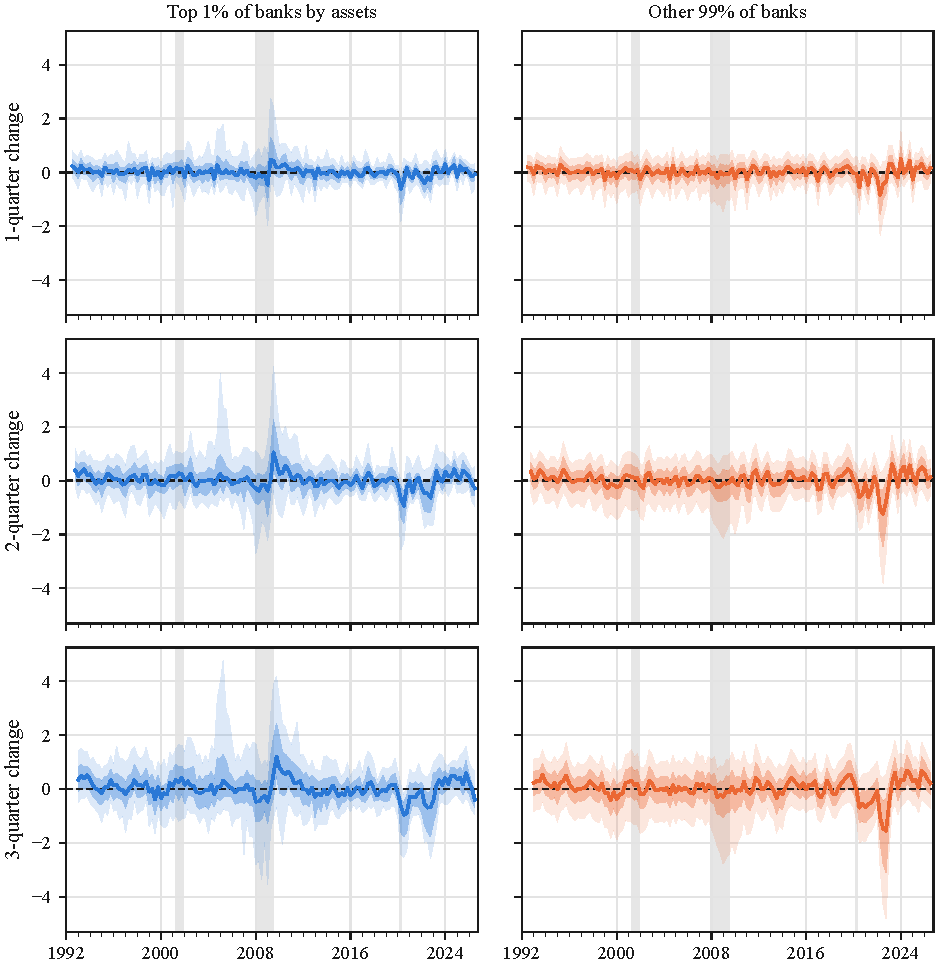
\includegraphics[width=\textwidth]{size_diff_equity_ratio_bare.pdf}
  \caption{Change in equity capital to assets (percentage points).}
  \label{fig:equity}
  \vspace{0.2em}
  \begin{minipage}{\textwidth}\footnotesize
    \textit{Notes:} Percentage-point change in each bank's ratio of total equity capital to total assets from $k$ quarters earlier. Bands as in Figure~\ref{fig:assets}. Shaded areas indicate NBER recessions. \textit{Source:} FDIC Statistics on Depository Institutions; author's calculations.
  \end{minipage}
\end{figure}

\begin{figure}[p]
  \centering
  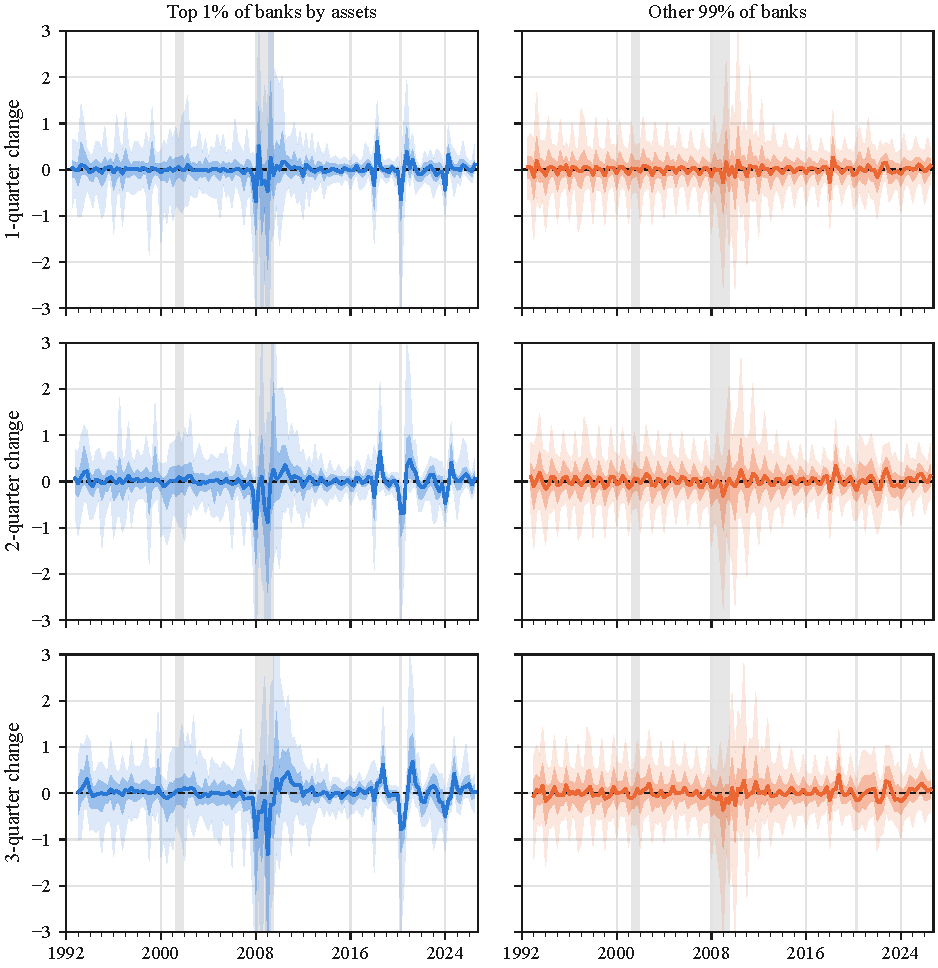
\includegraphics[width=\textwidth]{size_diff_roa_bare.pdf}
  \caption{Change in return on assets (percentage points).}
  \label{fig:roa}
  \vspace{0.2em}
  \begin{minipage}{\textwidth}\footnotesize
    \textit{Notes:} Percentage-point change in each bank's single-quarter, annualized ROA from $k$ quarters earlier (see Section~\ref{sec:data}). The vertical axis is capped at $\pm 3$, which clips the large-bank tails in 2008--09. Bands as in Figure~\ref{fig:assets}. Shaded areas indicate NBER recessions. \textit{Source:} FDIC Statistics on Depository Institutions; author's calculations.
  \end{minipage}
\end{figure}

\begin{figure}[p]
  \centering
  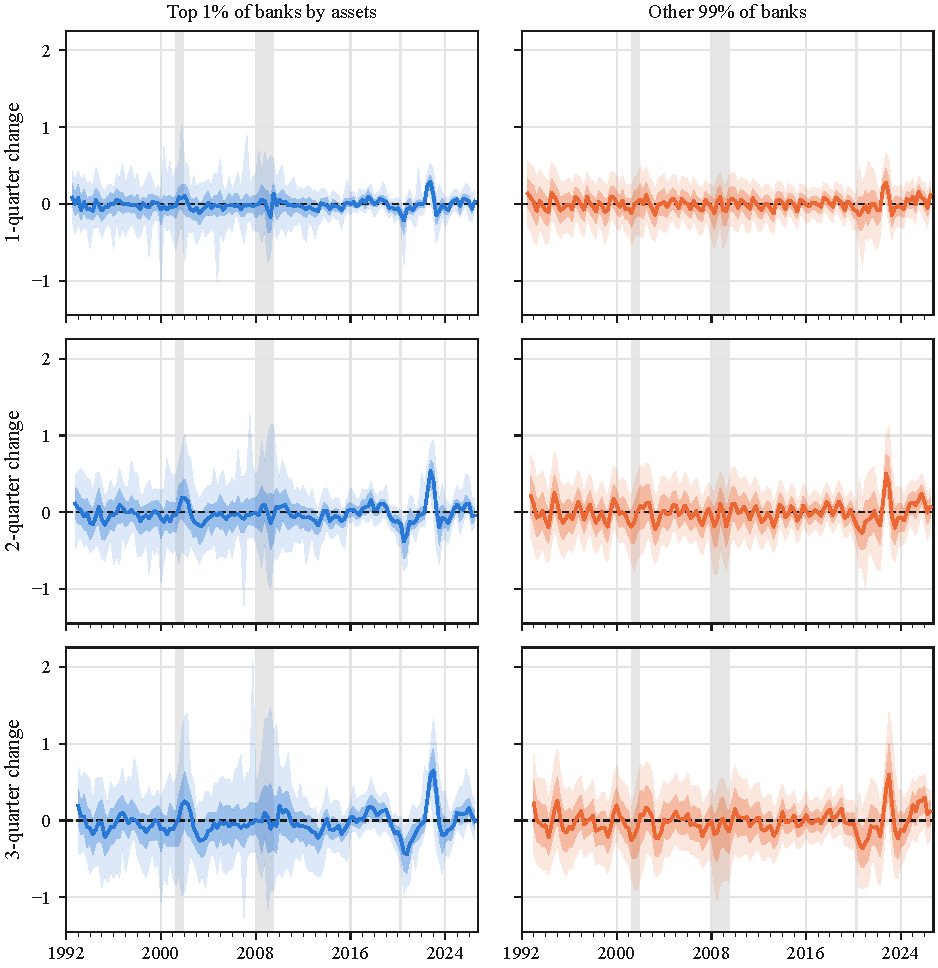
\includegraphics[width=\textwidth]{size_diff_nim_bare.pdf}
  \caption{Change in net interest margin (percentage points).}
  \label{fig:nim}
  \vspace{0.2em}
  \begin{minipage}{\textwidth}\footnotesize
    \textit{Notes:} Percentage-point change in each bank's single-quarter, annualized net interest margin from $k$ quarters earlier. Bands as in Figure~\ref{fig:assets}. Shaded areas indicate NBER recessions. \textit{Source:} FDIC Statistics on Depository Institutions; author's calculations.
  \end{minipage}
\end{figure}

\clearpage
% ---------------------------------------------------------------------------
\section{Symmetry and other distributional features}\label{sec:comments}

\subsection{Measuring symmetry}

Moment-based skewness is dominated by a handful of extreme observations, such as merger quarters, failing banks, and reporting errors, so all statistics here are built from the same quantiles plotted in the figures. For each group, variable, horizon and quarter,
\[
  \text{Bowley} = \frac{q_{75} + q_{25} - 2q_{50}}{q_{75} - q_{25}}, \qquad
  \text{Kelley} = \frac{q_{90} + q_{10} - 2q_{50}}{q_{90} - q_{10}}, \qquad
  \text{IQR} = q_{75} - q_{25}.
\]
Both skewness measures lie in $[-1, 1]$ and equal zero for a symmetric distribution. A positive value means the upper side of the distribution is stretched relative to the lower side. Bowley skewness describes the middle half of banks, while Kelley skewness reaches into the tails. Each quarterly statistic is averaged over expansion quarters (124--127, depending on the horizon) and, separately, over the 11 quarters that overlap an NBER recession: 2001Q2--Q4, 2008Q1--2009Q2 and 2020Q1--Q2. Tables~\ref{tab:bowley}--\ref{tab:median} report the results.

\begin{table}[htbp]
  \centering
  \begin{threeparttable}
    \caption{Quartile (Bowley) skewness of $k$-quarter changes}
    \label{tab:bowley}
    \small
    \begin{tabular}{@{}lcccc@{}}
\toprule
 & \multicolumn{2}{c}{Top 1\% of banks} & \multicolumn{2}{c}{Other 99\% of banks} \\
\cmidrule(lr){2-3} \cmidrule(l){4-5}
 & Expansion & Recession & Expansion & Recession \\
\midrule
\multicolumn{5}{l}{\textit{Total assets (\%)}} \\
\quad $k=1$ & 0.13 & 0.09 & 0.08 & 0.09 \\
\quad $k=2$ & 0.17 & 0.15 & 0.09 & 0.11 \\
\quad $k=3$ & 0.19 & 0.22 & 0.11 & 0.14 \\
\addlinespace
\multicolumn{5}{l}{\textit{Equity to assets (pp)}} \\
\quad $k=1$ & 0.00 & 0.02 & $-$0.04 & $-$0.09 \\
\quad $k=2$ & 0.01 & $-$0.02 & $-$0.04 & $-$0.10 \\
\quad $k=3$ & 0.00 & $-$0.09 & $-$0.03 & $-$0.11 \\
\addlinespace
\multicolumn{5}{l}{\textit{Return on assets (pp)}} \\
\quad $k=1$ & 0.02 & $-$0.05 & 0.00 & $-$0.03 \\
\quad $k=2$ & $-$0.01 & $-$0.04 & 0.00 & $-$0.04 \\
\quad $k=3$ & $-$0.02 & $-$0.06 & 0.01 & $-$0.10 \\
\addlinespace
\multicolumn{5}{l}{\textit{Net interest margin (pp)}} \\
\quad $k=1$ & 0.02 & $-$0.04 & 0.00 & $-$0.03 \\
\quad $k=2$ & $-$0.01 & $-$0.04 & 0.00 & $-$0.05 \\
\quad $k=3$ & 0.01 & $-$0.03 & 0.00 & $-$0.07 \\
\bottomrule
\end{tabular}

    \begin{tablenotes}[flushleft]\footnotesize
      \item \textit{Notes:} Average across quarters of $(q_{75}+q_{25}-2q_{50})/(q_{75}-q_{25})$ computed within each size group and quarter. Zero indicates a symmetric middle half. Recession quarters are those overlapping an NBER recession (11 quarters); all other quarters (124--127, depending on the horizon) are expansion quarters.
    \end{tablenotes}
  \end{threeparttable}
\end{table}

\begin{table}[htbp]
  \centering
  \begin{threeparttable}
    \caption{Decile (Kelley) skewness of $k$-quarter changes}
    \label{tab:kelley}
    \small
    \begin{tabular}{@{}lcccc@{}}
\toprule
 & \multicolumn{2}{c}{Top 1\% of banks} & \multicolumn{2}{c}{Other 99\% of banks} \\
\cmidrule(lr){2-3} \cmidrule(l){4-5}
 & Expansion & Recession & Expansion & Recession \\
\midrule
\multicolumn{5}{l}{\textit{Total assets (\%)}} \\
\quad $k=1$ & 0.24 & 0.18 & 0.16 & 0.20 \\
\quad $k=2$ & 0.32 & 0.30 & 0.20 & 0.26 \\
\quad $k=3$ & 0.37 & 0.36 & 0.24 & 0.32 \\
\addlinespace
\multicolumn{5}{l}{\textit{Equity to assets (pp)}} \\
\quad $k=1$ & 0.01 & 0.04 & $-$0.09 & $-$0.19 \\
\quad $k=2$ & 0.04 & $-$0.07 & $-$0.08 & $-$0.22 \\
\quad $k=3$ & 0.05 & $-$0.12 & $-$0.07 & $-$0.25 \\
\addlinespace
\multicolumn{5}{l}{\textit{Return on assets (pp)}} \\
\quad $k=1$ & $-$0.01 & $-$0.02 & 0.00 & $-$0.04 \\
\quad $k=2$ & $-$0.02 & $-$0.13 & 0.01 & $-$0.08 \\
\quad $k=3$ & $-$0.03 & $-$0.13 & 0.02 & $-$0.15 \\
\addlinespace
\multicolumn{5}{l}{\textit{Net interest margin (pp)}} \\
\quad $k=1$ & 0.02 & 0.02 & 0.00 & $-$0.06 \\
\quad $k=2$ & 0.03 & 0.04 & 0.00 & $-$0.10 \\
\quad $k=3$ & 0.02 & 0.03 & 0.01 & $-$0.13 \\
\bottomrule
\end{tabular}

    \begin{tablenotes}[flushleft]\footnotesize
      \item \textit{Notes:} Average across quarters of $(q_{90}+q_{10}-2q_{50})/(q_{90}-q_{10})$. Regimes as in Table~\ref{tab:bowley}.
    \end{tablenotes}
  \end{threeparttable}
\end{table}

\begin{table}[htbp]
  \centering
  \begin{threeparttable}
    \caption{Interquartile range of $k$-quarter changes}
    \label{tab:iqr}
    \small
    \begin{tabular}{@{}lcccc@{}}
\toprule
 & \multicolumn{2}{c}{Top 1\% of banks} & \multicolumn{2}{c}{Other 99\% of banks} \\
\cmidrule(lr){2-3} \cmidrule(l){4-5}
 & Expansion & Recession & Expansion & Recession \\
\midrule
\multicolumn{5}{l}{\textit{Total assets (\%)}} \\
\quad $k=1$ & 4.68 & 6.32 & 4.37 & 5.24 \\
\quad $k=2$ & 8.05 & 9.93 & 6.57 & 7.81 \\
\quad $k=3$ & 11.85 & 14.36 & 8.50 & 9.99 \\
\addlinespace
\multicolumn{5}{l}{\textit{Equity to assets (pp)}} \\
\quad $k=1$ & 0.49 & 0.86 & 0.56 & 0.68 \\
\quad $k=2$ & 0.75 & 1.20 & 0.81 & 0.95 \\
\quad $k=3$ & 0.98 & 1.42 & 0.98 & 1.15 \\
\addlinespace
\multicolumn{5}{l}{\textit{Return on assets (pp)}} \\
\quad $k=1$ & 0.36 & 1.09 & 0.47 & 0.61 \\
\quad $k=2$ & 0.44 & 1.20 & 0.52 & 0.70 \\
\quad $k=3$ & 0.49 & 1.19 & 0.56 & 0.72 \\
\addlinespace
\multicolumn{5}{l}{\textit{Net interest margin (pp)}} \\
\quad $k=1$ & 0.20 & 0.33 & 0.27 & 0.35 \\
\quad $k=2$ & 0.29 & 0.48 & 0.36 & 0.49 \\
\quad $k=3$ & 0.37 & 0.65 & 0.42 & 0.58 \\
\bottomrule
\end{tabular}

    \begin{tablenotes}[flushleft]\footnotesize
      \item \textit{Notes:} Average across quarters of $q_{75}-q_{25}$, in percent for total assets and percentage points otherwise. Regimes as in Table~\ref{tab:bowley}.
    \end{tablenotes}
  \end{threeparttable}
\end{table}

\begin{table}[htbp]
  \centering
  \begin{threeparttable}
    \caption{Median $k$-quarter change}
    \label{tab:median}
    \small
    \begin{tabular}{@{}lcccc@{}}
\toprule
 & \multicolumn{2}{c}{Top 1\% of banks} & \multicolumn{2}{c}{Other 99\% of banks} \\
\cmidrule(lr){2-3} \cmidrule(l){4-5}
 & Expansion & Recession & Expansion & Recession \\
\midrule
\multicolumn{5}{l}{\textit{Total assets (\%)}} \\
\quad $k=1$ & 1.44 & 1.67 & 1.11 & 2.20 \\
\quad $k=2$ & 3.23 & 4.00 & 2.42 & 3.95 \\
\quad $k=3$ & 5.26 & 6.44 & 3.74 & 5.64 \\
\addlinespace
\multicolumn{5}{l}{\textit{Equity to assets (pp)}} \\
\quad $k=1$ & 0.02 & $-$0.07 & 0.03 & $-$0.11 \\
\quad $k=2$ & 0.03 & $-$0.10 & 0.04 & $-$0.14 \\
\quad $k=3$ & 0.05 & $-$0.18 & 0.04 & $-$0.14 \\
\addlinespace
\multicolumn{5}{l}{\textit{Return on assets (pp)}} \\
\quad $k=1$ & 0.01 & $-$0.09 & 0.01 & $-$0.02 \\
\quad $k=2$ & 0.02 & $-$0.21 & 0.01 & $-$0.06 \\
\quad $k=3$ & 0.03 & $-$0.37 & 0.02 & $-$0.11 \\
\addlinespace
\multicolumn{5}{l}{\textit{Net interest margin (pp)}} \\
\quad $k=1$ & $-$0.01 & $-$0.01 & 0.00 & $-$0.03 \\
\quad $k=2$ & $-$0.02 & $-$0.02 & 0.00 & $-$0.08 \\
\quad $k=3$ & $-$0.03 & $-$0.02 & $-$0.01 & $-$0.11 \\
\bottomrule
\end{tabular}

    \begin{tablenotes}[flushleft]\footnotesize
      \item \textit{Notes:} Average across quarters of the within-group median change, in percent for total assets and percentage points otherwise. Regimes as in Table~\ref{tab:bowley}.
    \end{tablenotes}
  \end{threeparttable}
\end{table}

\subsection{Symmetry by variable}

\paragraph{Total assets: persistent right skew.}
Asset changes are the only outcome that is skewed in the same direction in every cell of Tables~\ref{tab:bowley} and~\ref{tab:kelley}. The skew is positive, with Bowley coefficients of 0.08--0.22 and Kelley coefficients of 0.16--0.37. Balance sheets can grow discretely, through an acquisition or a deposit inflow, but rarely shrink that way, so the upper tail is long. The skew is stronger for large banks (expansion Kelley 0.24--0.37 versus 0.16--0.24), consistent with acquisitions being concentrated among the largest institutions. The median asset change is \emph{higher} in recessions for both groups, for example $2.2\%$ versus $1.1\%$ per quarter for other banks at $k=1$ (Table~\ref{tab:median}). This mostly reflects deposit inflows in 2008--09 and especially 2020Q2, when an unusual deposit surge landed inside a two-quarter recession window; it should not be read as a general pattern.

\paragraph{Equity to assets: a negative skew that deepens in recessions for smaller banks.}
For large banks, changes in the equity ratio are close to symmetric in expansions, with both coefficients within $0.05$ of zero at every horizon. For other banks they are mildly negatively skewed even in expansions: a minority of banks lose capital quickly, while gains accumulate slowly. In recessions the other-bank Kelley coefficient roughly doubles in magnitude, to $-0.19$ at $k=1$ and $-0.25$ at $k=3$. The lower tail, meaning banks whose capital is eroding, is what moves. Large banks develop a comparable negative skew only at the three-quarter horizon ($-0.12$). Their larger recession change is in \emph{dispersion}: the interquartile range rises by about 75\% (0.50 to 0.87 pp at $k=1$), against about 20\% for other banks (Table~\ref{tab:iqr}). Figure~\ref{fig:equity} shows the source: large banks were recapitalized in 2009, while other banks show a sharp, broad-based decline in 2022, when rising interest rates reduced the value of their securities holdings.

\paragraph{Return on assets: symmetric in good times, left-skewed in bad times.}
In expansions, ROA changes are almost perfectly symmetric in both groups ($|\text{Bowley}| \le 0.03$). This is what one expects of a stationary ratio whose quarter-to-quarter movements are mostly transitory noise. Recessions break the symmetry: skewness turns negative in both groups and grows with the horizon, reaching a Kelley coefficient of about $-0.13$ to $-0.15$ at $k=3$. The two groups differ mainly in location and spread. The large-bank median falls by $0.37$ pp over three quarters of a recession, against $0.11$ pp for other banks. The large-bank interquartile range roughly triples, from 0.36 to 1.08 pp at $k=1$, while the other-bank range rises only from 0.47 to 0.61 pp. The ordering therefore reverses. \emph{In expansions large banks have the more tightly clustered profitability changes; in recessions they have the more dispersed ones.} Several large banks absorbed heavy losses in 2008--09 while others did not, whereas small-bank losses were more evenly spread.

\paragraph{Net interest margin: symmetric for large banks, left-skewed for small banks in recessions.}
NIM changes are symmetric in expansions for both groups. In recessions, other banks develop a negative skew (Kelley $-0.06$ at $k=1$, $-0.13$ at $k=3$) and a falling median ($-0.11$ pp at $k=3$). Large banks' NIM distribution stays close to symmetric and its median barely moves ($-0.02$ pp). As policy rates are cut, margins compress most for the banks that are least able to reprice their liabilities, and those banks sit in the lower tail of the other-bank distribution. Both groups show the same 2022--23 rise and subsequent reversal in Figure~\ref{fig:nim} as rates increased and deposit costs caught up.

\subsection{Other important concepts}

\paragraph{Horizon scaling reveals persistence.}
If quarterly changes were independent and identically distributed, the spread of $k$-quarter changes would grow roughly in proportion to $\sqrt{k}$, so the three-quarter interquartile range would be about $\sqrt{3} \approx 1.73$ times the one-quarter range. The expansion-period ratios for other banks in Table~\ref{tab:iqr} differ sharply by variable: 1.95 for assets, 1.76 for the equity ratio, 1.57 for NIM, and 1.20 for ROA. Asset growth is persistent: banks that grow keep growing. The equity ratio behaves close to a random walk. ROA changes are largely transitory and mean-reverting, so a bad quarter tends to be followed by a better one. For large banks the asset ratio is higher still (2.52), again pointing to acquisition-driven growth.

\paragraph{A distribution of changes is not a change in the distribution.}
The fan charts show the distribution of \emph{within-bank} changes $\Delta_k x_{it}$. They are not differences between cross-sectional percentiles at $t$ and $t-k$. A median change of zero is compatible with the whole cross-section drifting apart: some banks rise, others fall, and dispersion in levels grows. Statements about inequality \emph{across} banks, such as whether large banks become more profitable relative to small banks, require the level distributions, not these figures.

\paragraph{Grouping on current size selects on growth.}
Because group membership is determined by assets at $t$, a bank that crossed into the top 1\% through rapid growth or an acquisition is, mechanically, a large bank with a large asset change. This inflates the upper tail and the right skew of large-bank asset growth, and to a lesser extent anything correlated with growth. A robustness check is to assign groups using assets at $t-k$, or to fix membership at the start of each episode.

\paragraph{Survivorship and entry.}
A change is defined only if the bank reports in both $t-k$ and $t$. Banks that fail or are absorbed drop out after their last filing, so the very worst outcomes, such as a bank's final quarter before closure, can be missing from the lower tail. New charters enter only after $k$ quarters. Both effects matter most in 2008--10, when several hundred institutions failed. The recession lower tails in Tables~\ref{tab:bowley}--\ref{tab:kelley} should therefore be read as lower bounds on the true severity.

\paragraph{Small groups make tails noisy.}
The large-bank group contains 42--144 banks, so its 10th and 90th percentiles are set by roughly the 4th to 14th most extreme institution. Kelley skewness for large banks, and the outer band in each large-bank panel, carry considerably more sampling noise than the corresponding other-bank statistics. That group has several thousand banks per quarter. Differences in Kelley skewness between groups of less than about 0.1 should not be over-interpreted.

\paragraph{Few recession quarters, one dominant episode.}
Only 11 of 138 quarters overlap a recession, and 6 of them fall in 2008--09. The recession columns of the tables are therefore mostly a description of the financial crisis. The 2001 recession barely registers in the bank data, and the 2020 recession is only two quarters long and is confounded by pandemic-era deposit inflows and loan-loss provisioning.

\paragraph{Overlapping horizons and seasonality.}
The two- and three-quarter changes in adjacent quarters share most of their underlying data, so they are smoother and strongly serially correlated. They are not independent evidence. Single-quarter ROA also retains a genuine fourth-quarter pattern, because banks book provisions, write-downs and year-end adjustments in Q4. This produces the regular sawtooth in the other-bank panels of Figures~\ref{fig:roa} and~\ref{fig:nim}. Four-quarter changes, or seasonally adjusting before differencing, would remove it.

\paragraph{Axis caps.}
The vertical axes of Figures~\ref{fig:assets} and~\ref{fig:roa} are truncated to keep the medians and inner bands legible. The statistics in Tables~\ref{tab:bowley}--\ref{tab:median} are computed from the full, untruncated quantiles.

\end{document}
